%%%% CS553 Cryptography Term Paper TEMPLATE %%%%

%%%% 1. DOCUMENTCLASS %%%%
\documentclass[preprint]{transcrypto}
%%%% NOTES:
% - Change "submission" to "final" for final version
% - Add "spthm" for LNCS-like theorems


%%%% 2. PACKAGES %%%%
\usepackage{lipsum} % Example package -- can be removed
% \usepackage{algorithm}
% \usepackage{algorithmic}
% \usepackage{algpseudocode}
% \usepackage{algcompatible}
% \documentclass[]{scrbook}
\usepackage[T1]{fontenc}
\usepackage[english]{babel}
% \usepackage{algorithm,algorithmicx,algpseudocode}
\usepackage[ruled,vlined]{algorithm2e}
\usepackage{amssymb}
\usepackage{enumitem}
% \usepackage{algorithm}
% \usepackage{arevmath}     % For math symbols
% \usepackage[noend]{algpseudocode}


\providecommand{\keywords}[1]
{
  \small	
  \textbf{\textit{Keywords---}} #1
}


%%%% 3. AUTHOR, INSTITUTE %%%%
\author{Meghana Varanasi\inst{1} \and Shreya Gundu\inst{2} \and Debajyoti Halder\inst{3}}
\institute{
  IIT Bhilai, Raipur, India, \email{meghana@iitbhilai.ac.in}
  \and
  IIT Bhilai, Raipur, India, \email{gundus@iitbhilai.ac.in}
  \and
  IIT Bhilai, Raipur, India, \email{debajyotih@iitbhilai.ac.in}
}
%%%% NOTES:
% - We need a city name for indexation purpose, even if it is redundant
%   (eg: University of Atlantis, Atlantis, Atlantis)
% - \inst{} can be omitted if there is a single institute,
%   or exactly one institute per author


%%%% 4. TITLE %%%%
\title{Implementation and Analysis of Mysterion}
%%%% NOTES:
% - If the title is too long, or includes special macro, please
%   provide a "running title" as optional argument: \title[Short]{Long}
% - You can provide an optional subtitle with \subtitle.

\begin{document}

\maketitle
\begin{abstract}
  Mysterion is an instance of XLS-design which is a family of cipher with efficient bitslice implementation against side channel attack. We discuss Mysterion and its security against various attacks including invariant subspace attack and boomerang attack which is due to the XLS-design, a massive upgrade from LS-designs. We discuss the faults in LS-design and how combining Super S-boxes with ShiftColumns prevented attacks and gave sufficient security margin to Mysterion through XLS-design. A simple block cipher can still be very much secure against physical attacks.

\end{abstract}
%%%% 5. KEYWORDS %%%%
% \keywords{Mysterion \and XLS-design \and Invariant Subspace Attack}


%%%% 6. ABSTRACT %%%%

\tableofcontents
\newpage

%%%% 7. PAPER CONTENT %%%%
\section{Introduction}

LS-designs presented us with efficient bit slicing. They were combinations of linear diffusion L-boxes and non-linear bitslice S-boxes. However LS-designs were susceptible to invariant subspace attack which led to doubts on the proposed instances of LS-designs. XLS-designs prevented the attacks with heuristic changes. A better choice of round constants prevented the propagation of invariant subspace for the S-boxes or L-boxes. We now have an eXtensible LS-design. 
\\\\
In this paper we demonstrate Mysterion, an instance of XLS-design comprising of Super S-boxes, made of optimal components - 4-bit S-boxes and 32-bit L-boxes based on Maximum Distance Separable (MDS) code, and ShiftColumns operation. We show security margins of Mysterion and it's similarity with AES-like cipher because of the combined S-boxes and ShiftColumns design.

% Widely used primitives like the AES~\cite{AES} do not have perfect
% security, and can be analysed with linear
% cryptanalysis~\cite{EC:Matsui93}, differential
% cryptanalysis~\cite{JC:BihSha91}, or differential power
% analysis~\cite{C:KocJafJun99}.  We show that the One-Time-Pad is
% unconditionally secure in \autoref{sec:main}.

\section{Mathematics}
\label{sec:math}
\begin{enumerate}
    \item \textbf{Galios Field :} Galois field is a field that contains a finite number of elements. As with any field, a finite field is a set on which the operations of multiplication, addition, subtraction and division are defined and satisfy certain basic rules. The most common examples of finite fields are given by the integers mod $p$ when $p$ is a prime number.
    \item \textbf{Companion matrix :} In linear algebra, the Frobenius companion matrix of the monic polynomial
${\displaystyle p(t)=c_{0}+c_{1}t+\cdots +c_{n-1}t^{n-1}+t^{n}~,}$
is the square matrix defined as

     $$ C(p)={\begin{bmatrix}0&0&\dots &0&-c_{0}\\1&0&\dots &0&-c_{1}\\0&1&\dots &0&-c_{2}\\\vdots &\vdots &\ddots &\vdots &\vdots \\0&0&\dots &1&-c_{{n-1}}\end{bmatrix}} $$



    \item \textbf{MDS matrix :} An MDS matrix (Maximum Distance Separable) is a matrix representing a function with certain diffusion properties that have useful applications in cryptography. Technically, an m×n matrix A over a finite field K is an MDS matrix if it is the transformation matrix of a linear transformation $f(x)=Ax$ from Kn to Km such that no two different $(m+n)$-tuples of the form $(x,f(x))$ coincide in n or more components. Equivalently, the set of all $(m+n)$-tuples $(x,f(x))$ is an MDS code, i.e. a linear code that reaches the Singleton bound.
    \item \textbf{BCH code :} In coding theory, the BCH codes or Bose–Chaudhuri–Hocquenghem codes form a class of cyclic error-correcting codes that are constructed using polynomials over a finite field (also called Galois field).
    
\end{enumerate}
 
\section{xLS Design}
\label{sec:xLS}
\subsection{Bit Slicing}

There are 2 basic ideas behind bit slicing :
\begin{enumerate}
    \item converting the cipher into bit-wise operations (like the way we'd implement it in hardware)
    \item carrying out those bit wise operations in parallel (We show two implementations of the sbox, one just showing the bitwise operation on each 4 bit input as well as on a block (8x4 i.e.,applying it paralelly on 8 inputs of size 4 bits ))
\end{enumerate}
Bitwise slicing is efficent in the following cases :
\begin{enumerate}
    \item Bit shifts, rotations and other bit permutations
    \item Bitwise logical operations
    \item Addition and subtraction
    \item multiplication and division
    \item Table lookups
    \item Conditional code

\end{enumerate}
\subsection{LS and xLS Designs}

\subsubsection{Brief on LS Design}
\begin{center}
  
\includegraphics[]{ls.png}  
\end{center}
LS-designs, proposed at FSE 2014, aimed for efficient bitslice implementation. LS-designs, as it is obvious by the name, are combinations of linear diffusion L-boxes and non-liner bitslice S-boxes. 
\\\\
Among the two proposed instances - Robin (involutive cipher) and Fantomas (non-involutive cipher), involutive instance Robin is susceptible to an invariant subspace attack, and has lead to a weak key set of density $2^{-32}$. 
\\\\
The invariant subspace attack against Robin can be prevented with simple heuristics i.e. better choice of round constants. In order to avoid invariant subspaces for the S-boxes or L-boxes to be propagated through the rounds, the round constants should have varying bits (in bitslice representation).


\subsubsection{XLS Design - the difference}
\begin{center}
    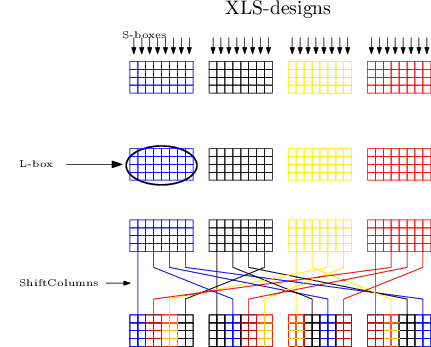
\includegraphics[]{xls.png} 
\end{center}
eXtensible LS (XLS) Design is based on 32-bit “Super S-Boxes” (4-bit S-boxes and 32-bit L-boxes based on a Maximum Distance Separable (MDS) code), which are further combined with additional ShiftColumns operation to obtain 128 and 256 bit ciphers. 
\\\\
AES also had a similar approach, using S-boxes and then combining with ShiftRows (also Mix Columns and round keys). However here bitslice is used rather than a block structure.
\\\\
Few differences pointers:
\begin{enumerate}
    \item its diffusion layer is not based on binary matrices anymore (non-binary MDS code is used with S-boxes with smaller bit sizes)
    \item it requires an additional ShiftColumns operations
\end{enumerate}

% \section{Specifications? \& Algos}
% \label{sec:Spec}
\section{Analysis}

\hrule height 1pt  \relax \vspace{5pt}
{\centering
\noindent\textbf{Algorithm :} XLS-design with $l \cdot s$ -bit L-boxes, $s$ -bit S-boxes and $b$ blocks\\} \vspace{3pt}
\hrule \relax
\begin{enumerate}[label=\arabic*:]
	\item $x \leftarrow P \oplus K$  \hfill $\triangleright$ $x$   is a $s.(l . b)$  bits matrix
	\item \textbf{for} $0 \leq r<N_{r}$ \textbf{do}
	\item$\quad$ \textbf{for} $0 \leq j<b$ \textbf{do}
	\item$\quad\quad$ \textbf{for} $0 \leq i<l$ \textbf{do}
	\item$\quad\quad\quad x[j, \star, i]=\mathrm{S}[x[j, \star, i]] ; \quad \quad \quad \quad \quad$ \hfill $\triangleright$ \textbf{S}-box layer
	\item$\quad\quad$ \textbf{for} $0 \leq j<b$ \textbf{do}
	\item$\quad\quad\quad x[j, \star, \star]=\mathrm{L}[x[j, \star, \star]]$ \hfill $\triangleright$
	\textbf{L}-box layer
	\item$\quad\quad$ \textbf{for} $0 \leq k<s$ \textbf{do}
	\item$\quad\quad\quad x[\star, k, \star]=$ Shift Columns $[x[\star, k, \star]]$ \hfill $\triangleright$
	\textbf{ShiftColumns} layer
	\item$\quad\quad x \leftarrow x \oplus K \oplus C(r)$ \hfill $\triangleright$
	Key and round constant addition return
	\item \textbf{return} $x$
\end{enumerate}

\hrule \relax

\subsection{Sbox}

Mysterion uses S-boxes that has bitslice representation with a combination of AND (also OR) and XOR gates. The class-13 S-box, as used by Mysterion, has a bitslice representation of 4 AND (precisely 3 AND and 1 OR) gates and 4 XOR gates. It has an algebraic degree of three and as shown below - differential probability $2^{-2}$ and linear probability $2^{-1}$
\\\\
Algorithm :




	\begin{algorithm}
        % \SetAlgoLined
       \textbf{Require:} 4 input bits ($A$,$B$,$C$,$D$)\\
\textbf{Ensure:} 4 output bits such as ($a$,$b$,$c$,$d$)= S($A$,$B$,$C$,$D$)\\
1: $a = A$ $\&$ $B$; \\
2: $a = a$ \textcircled{+} $C$ ;\\
3: $c = B$ | $C$ ; \\
4: $c = c$ \textcircled{+} $D$ ;\\
5: $d = a$ $\&$ $D$; \\
6: $d = d$ \textcircled{+} $A$ ;\\
7: $b = c$ $\&$ $A$; \\
8: $b = b$ \textcircled{+} $B$ ;\\
9: \textbf{return} $(a,b,c,d)$  \\
         \caption{S-box, bitslice representation}
        \end{algorithm}





\subsubsection{DDT}
As you can see from the table, the Differential probability = $\dfrac{4}{16}$ = $2^{-2}$
\begin{table}[!h]
\centering
\begin{tabular}{|c|c|c|c|c|c|c|c|c|c|c|c|c|c|c|c|}
\hline
 &
%   \textbf{0} &
  \textbf{1} &
  \textbf{2} &
  \textbf{3} &
  \textbf{4} &
  \textbf{5} &
  \textbf{6} &
  \textbf{7} &
  \textbf{8} &
  \textbf{9} &
  \textbf{a} &
  \textbf{b} &
  \textbf{c} &
  \textbf{d} &
  \textbf{e} &
  \textbf{f} \\ \hline
% \textbf{.} & 16 & . & . & . & . & . & . & . & . & . & . & . & . & . & . & . \\ \hline
 \textbf{1}&4&.&.&.&4&.&.&4&.&.&.&.&4&.&.\\\hline
\textbf{2}&.&.&.&4&.&4&.&.&.&2&2&2&2&.&.\\\hline
\textbf{3}&2&.&2&.&2&.&2&.&2&.&2&2&.&2&.\\\hline
\textbf{4}&.&.&.&.&.&.&.&4&4&2&2&.&.&2&2\\\hline
\textbf{5}&4&.&.&.&4&.&.&.&.&2&2&.&.&2&2\\\hline
\textbf{6}&.&4&.&4&.&.&.&.&.&.&.&2&2&2&2\\\hline
\textbf{7}&2&.&2&.&2&.&2&.&2&2&.&2&.&.&2\\\hline
\textbf{8}&.&4&4&.&.&4&4&.&.&.&.&.&.&.&.\\\hline
\textbf{9}&.&2&2&.&.&2&2&.&.&2&2&.&.&2&2\\\hline
\textbf{a}&.&.&.&4&.&.&4&.&.&2&2&2&2&.&.\\\hline
\textbf{b}&2&2&.&.&2&2&.&.&2&2&.&2&.&.&2\\\hline
\textbf{c}&.&.&.&.&.&.&.&4&4&2&2&.&.&2&2\\\hline
\textbf{d}&.&2&2&.&.&2&2&4&.&.&.&.&4&.&.\\\hline
\textbf{e}&.&.&4&4&.&.&.&.&.&.&.&2&2&2&2\\\hline
\textbf{f}&2&2&.&.&2&2&.&.&2&.&2&2&.&2&.\\\hline
\end{tabular}
\caption{DDT of Sbox}
\end{table}

\subsubsection{LAT}
As you can see from the table, the Linear probability = $\dfrac{4}{8}$ = $2^{-1}$
\\
\begin{table}[!h]
\centering
\begin{tabular}{|c|c|c|c|c|c|c|c|c|c|c|c|c|c|c|c|}
\hline
 &
  \textbf{1} &
  \textbf{2} &
  \textbf{3} &
  \textbf{4} &
  \textbf{5} &
  \textbf{6} &
  \textbf{7} &
  \textbf{8} &
  \textbf{9} &
  \textbf{a} &
  \textbf{b} &
  \textbf{c} &
  \textbf{d} &
  \textbf{e} &
  \textbf{f} \\ \hline
\textbf{1}&4&.&-4&.&.&.&.&.&4&.&4&.&.&.&.\\\hline
\textbf{2}&.&.&.&4&4&4&-4&.&.&.&.&.&.&.&.\\\hline
\textbf{3}&.&.&.&4&.&-4&.&.&.&.&.&.&4&.&4\\\hline
\textbf{4}&2&.&2&.&-2&.&-2&4&2&.&-2&.&2&4&-2\\\hline
\textbf{5}&2&.&2&.&2&.&2&4&2&.&-2&.&-2&-4&2\\\hline
\textbf{6}&-2&.&-2&.&2&.&2&4&-2&.&2&4&2&.&-2\\\hline
\textbf{7}&2&.&2&.&2&.&2&-4&2&.&-2&4&2&.&-2\\\hline
\textbf{8}&.&-4&.&2&-2&2&2&.&.&4&.&2&-2&2&2\\\hline
\textbf{9}&4&.&.&-2&2&2&2&.&-4&.&.&-2&2&2&2\\\hline
\textbf{a}&.&4&.&-2&2&-2&-2&.&.&4&.&2&-2&2&2\\\hline
\textbf{b}&.&.&4&2&2&-2&2&.&.&.&4&-2&-2&2&-2\\\hline
\textbf{c}&-2&4&-2&2&.&2&4&.&2&.&-2&-2&.&2&.\\\hline
\textbf{d}&-2&.&2&-2&.&2&.&.&2&-4&2&2&.&2&4\\\hline
\textbf{e}&2&4&2&2&-4&2&.&.&-2&.&2&2&.&-2&.\\\hline
\textbf{f}&-2&.&2&-2&.&2&.&.&2&4&2&-2&4&-2&.\\\hline
\end{tabular}
\caption{LAT of Sbox}
\end{table}

\subsection{Lbox}
\begin{center}
    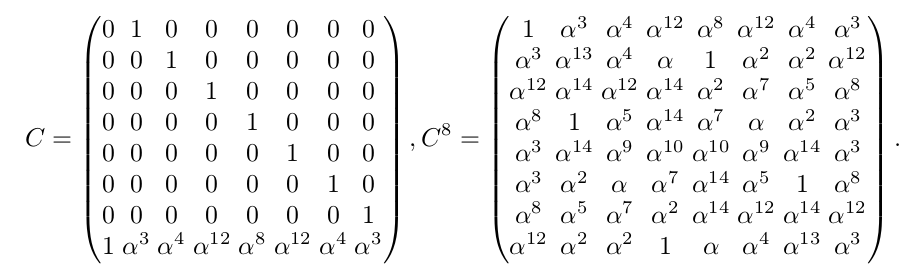
\includegraphics[scale=0.33]{l-box.png}\\
    
\end{center}
\begin{center}
    $C$ is the companion matrix of the polynomial\\
    $C^{8}$ is the underlying matrix of the Mysterion l-box
\end{center}

Mysterion Lbox uses linear transformation. The paper by Augot and Finiasz$^{[9]}$ proposes an algorithm which finds recursive MDS diffusion layers using shortened BCH codes. What this algorithm does is it takes degree of the polynomial k (hence the size of the companion matrices), and the field size $q = 2^s$ as parameters, and provides all the polynomials of degree k over $F_{2^s}$ such as their companion matrices raised to the power k gives MDS diffusion layers. \\ \\
% This algorithm provides all the polynomials of degree k over Galois Field of size $2^{s}$ such that their companion matrices when raised to the power of k gives MDS diffusion layers. \\
Selected polynomial, obtained after this is run using Magma code with parameters k = 8 and s = 4, has its coefficients in $\mathbb{F}_{2^{4}}$ is $\mathrm{P}(\mathrm{X})=\mathrm{X}^{8}+\alpha^{3} \cdot \mathrm{X}^{7}+\alpha^{4} \cdot \mathrm{X}^{6}+\alpha^{12} \cdot \mathrm{X}^{5}+\alpha^{8} \cdot \mathrm{X}^{4}+\alpha^{12} \cdot \mathrm{X}^{3}+\alpha^{4} \cdot \mathrm{X}^{2}+\alpha^{3} \cdot \mathrm{X}+1$.
Its differential and linear branch number equal to 9. 
\\ \\
Its purpose is to diffuse changes in the state. Because of this lbox, input change in one bit is diffused to entire state is just 2 rounds. LBox is implemented by multiplying the state with MDS matrix. The multiplying matrix was its companion matrix to the power eight therefore, we could replace one matrix multiplication by eight vector multiplications (This is what is done in the implementation). \\
\begin{center}
    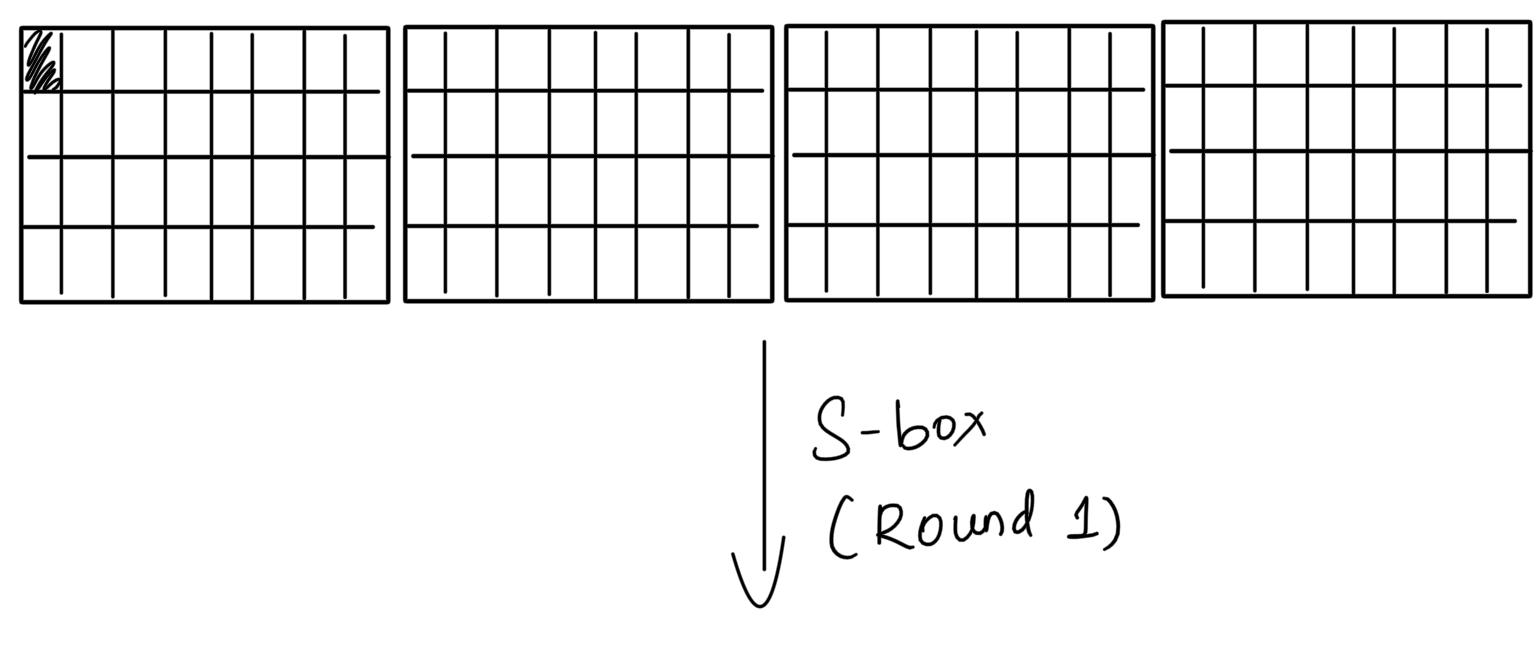
\includegraphics[scale=0.1]{PNG image.png}\\
    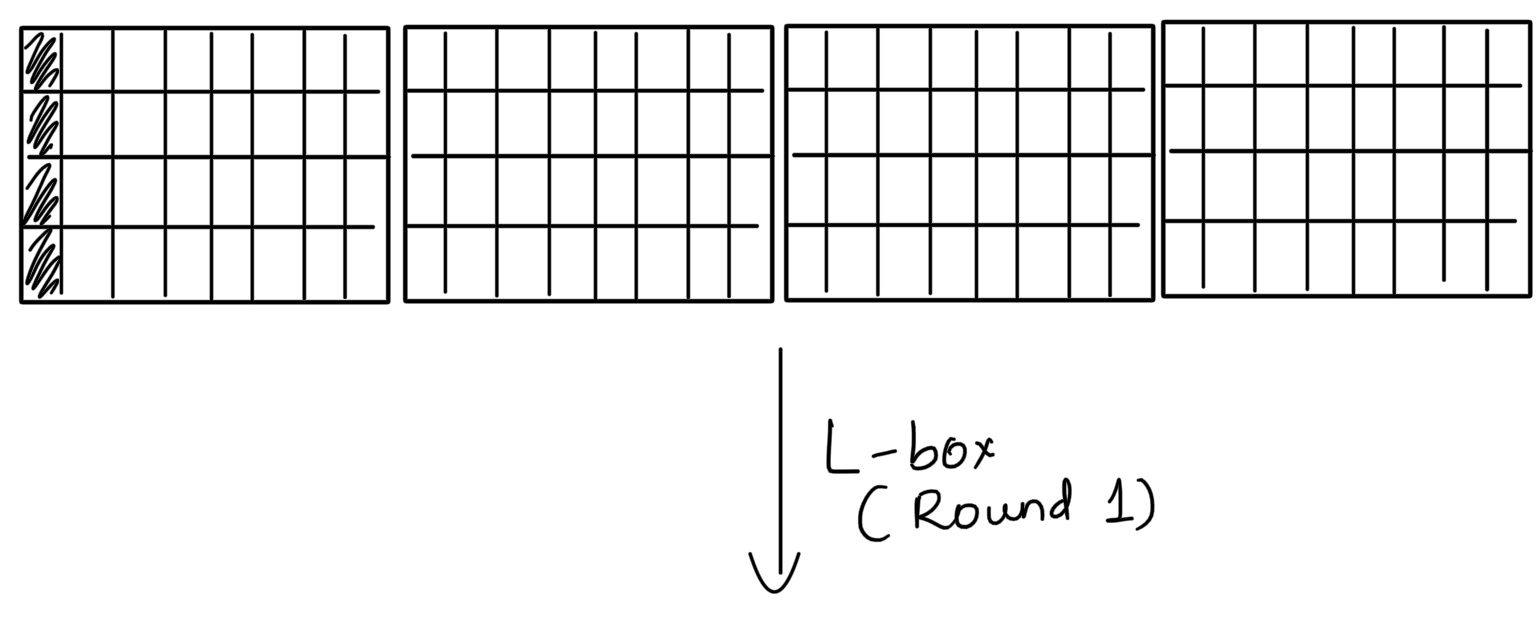
\includegraphics[scale=0.1]{PNG image-1.png}\\
    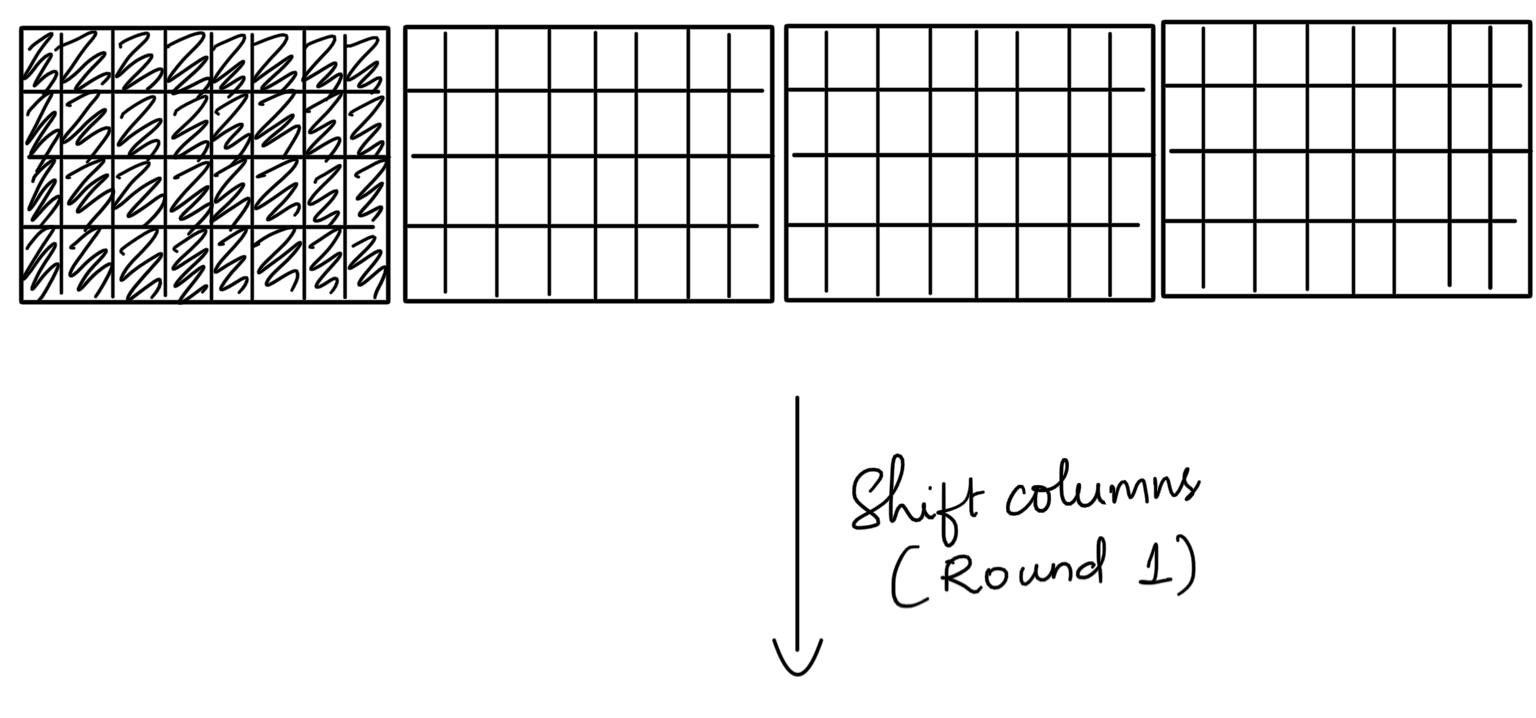
\includegraphics[scale=0.1]{PNG image-2.png}\\
    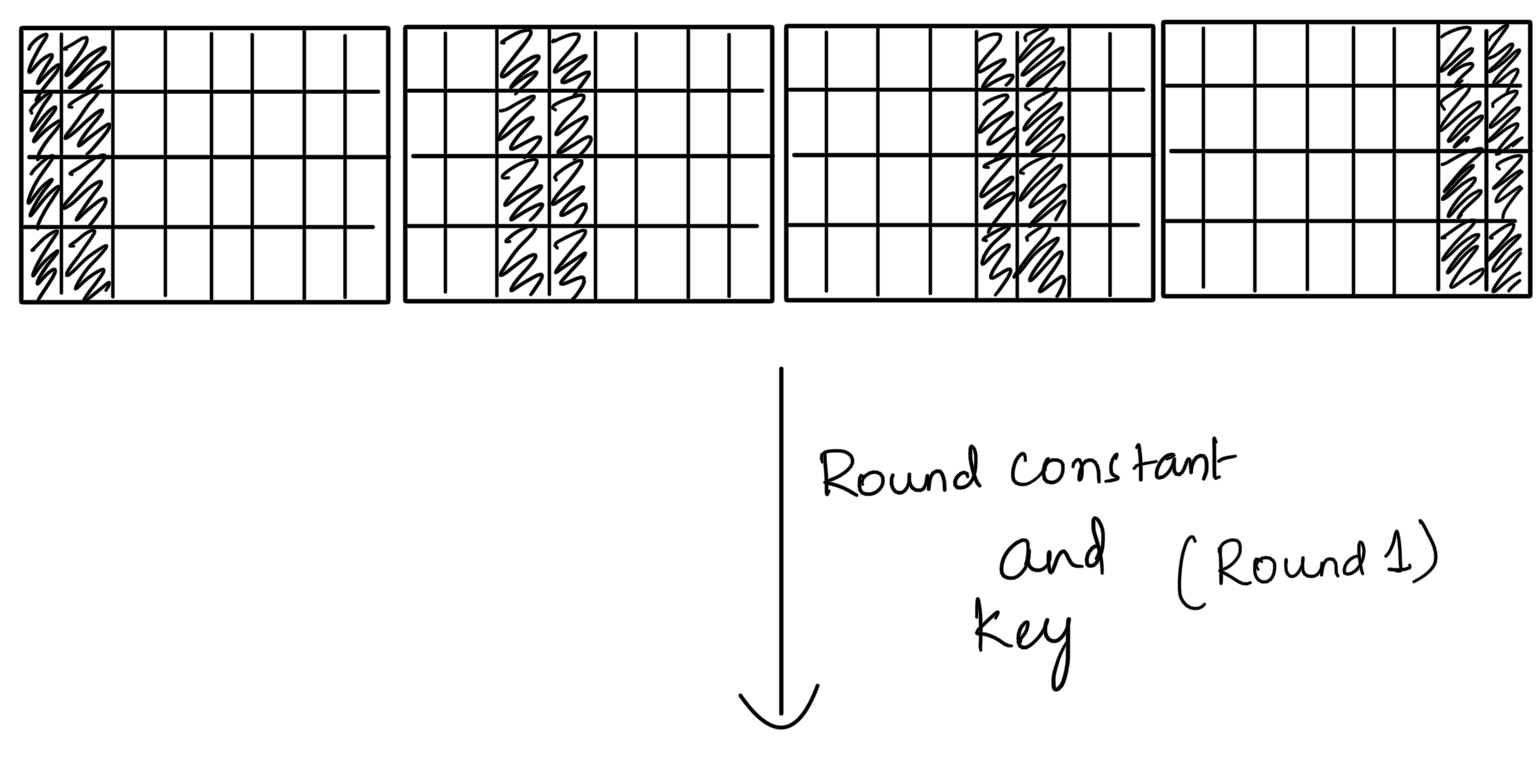
\includegraphics[scale=0.1]{PNG image-3.png}\\
    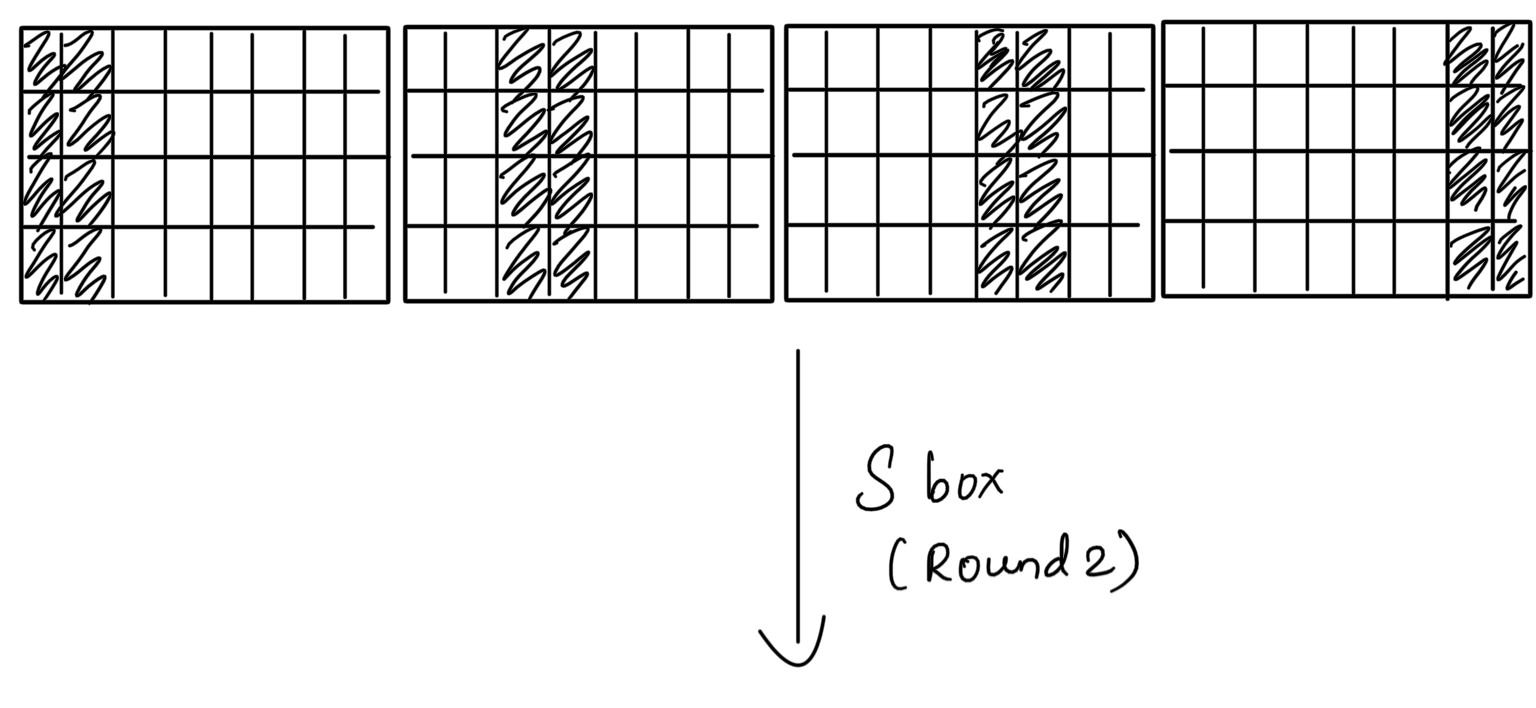
\includegraphics[scale=0.1]{PNG image-4.png}\\
    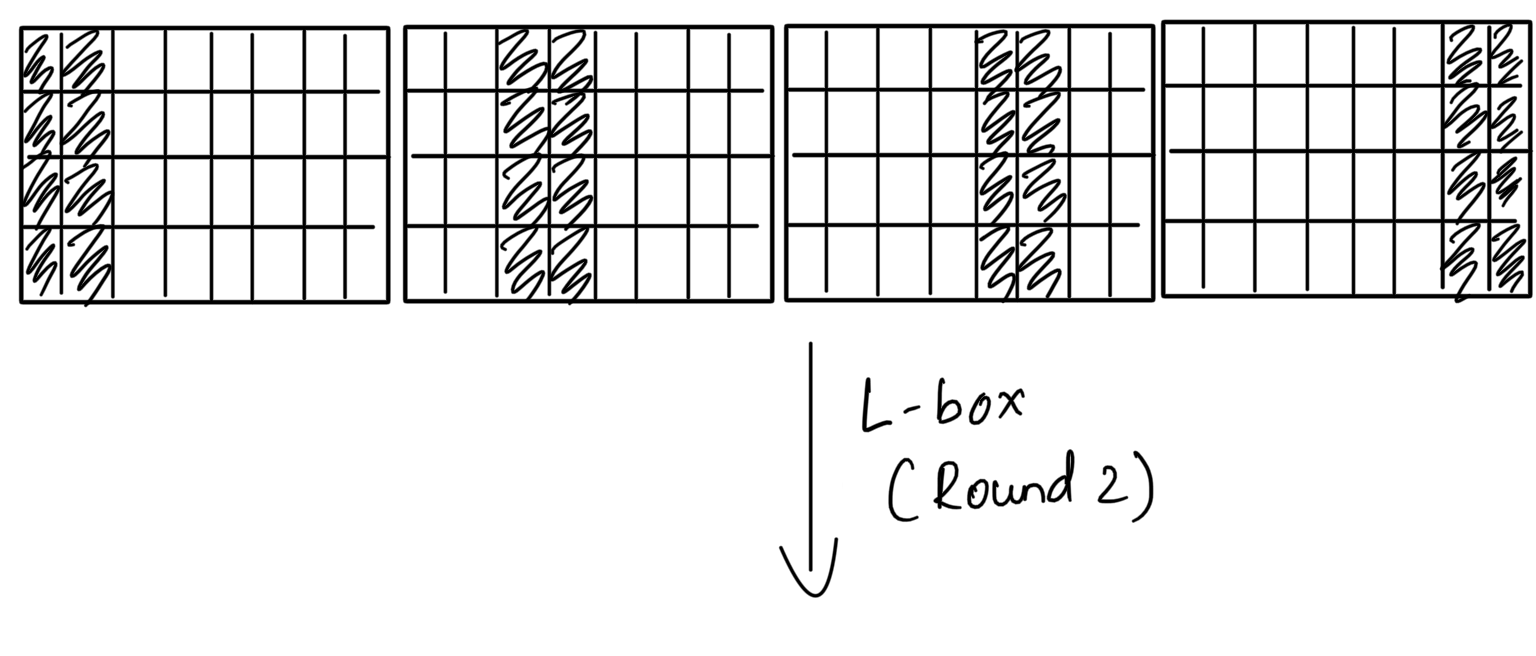
\includegraphics[scale=0.1]{PNG image-5.png}\\
    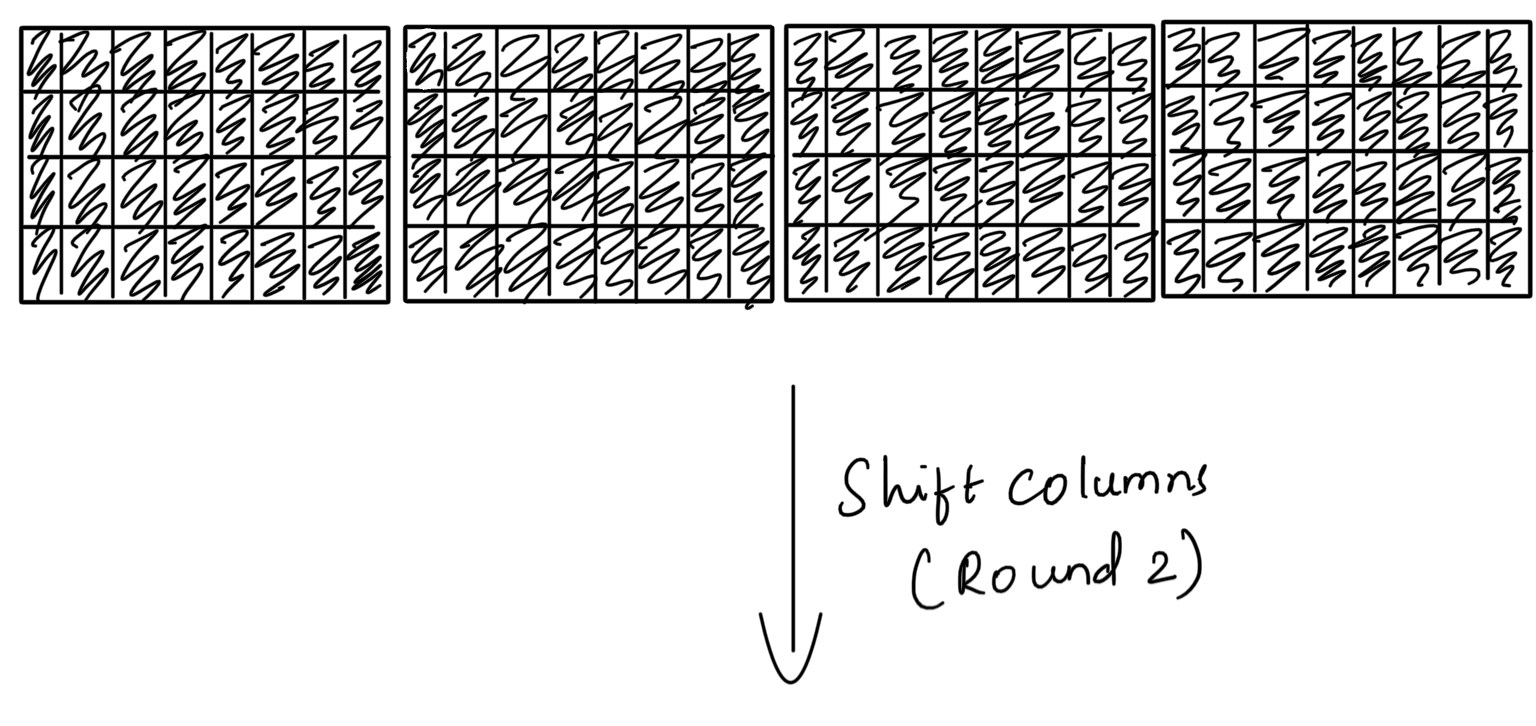
\includegraphics[scale=0.1]{PNG image-6.png}\\
    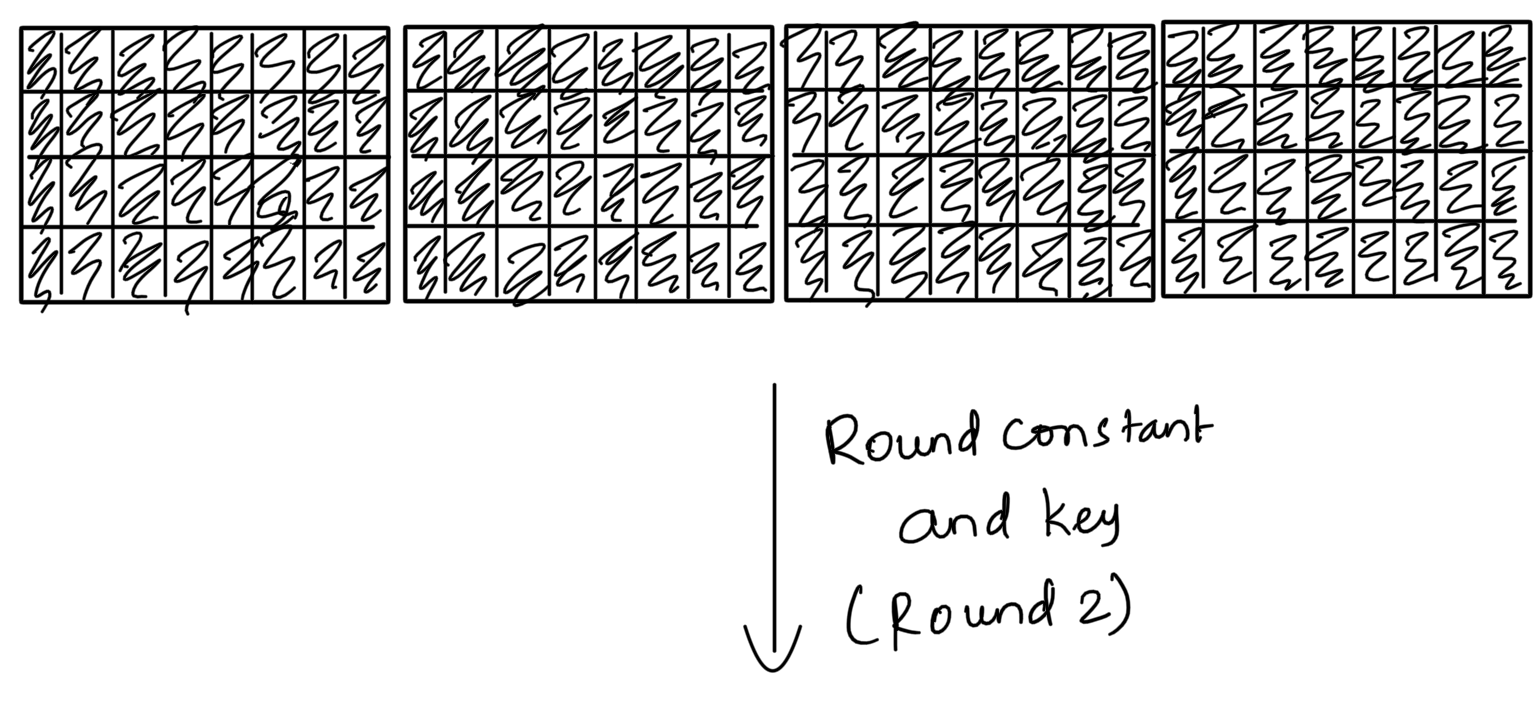
\includegraphics[scale=0.1]{PNG image-7.png}\\
    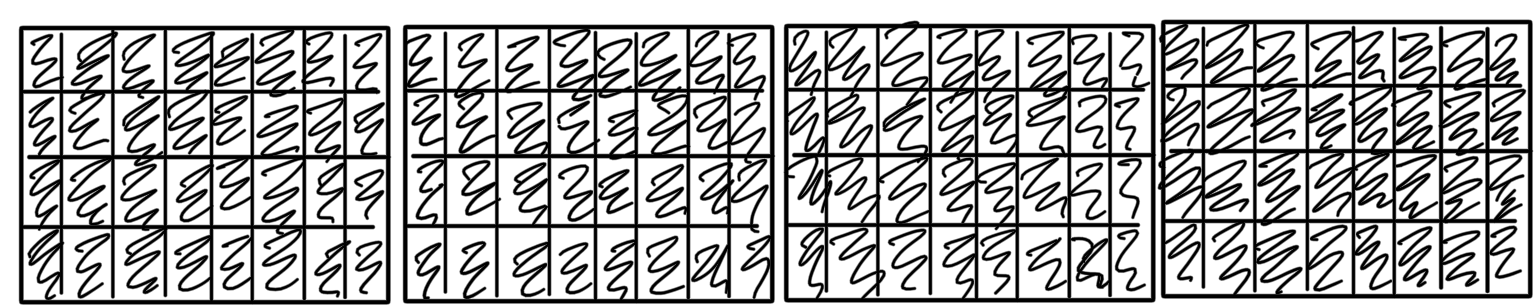
\includegraphics[scale=0.1]{PNG image-8.png}\\
\end{center}

% To obtain an 8 $\times$ 8 MDS matrix over a field size $2^{4}$ we assume $k = 8$ and $s = 4$. The resultant diffusion layer has an MDS code $[16,8,9]_{F_{2^{4}}}$ and therefore has both its differential and linear branch number equal to 9.
\subsection{Shift Columns}

In Mysterion-128, as there are 4 blocks (with  each block having 8 columns)  ShiftColumns acts on columns two by two. The first two columns of each block will be at the same position , the second two columns are moved by one block, the third two columns are moved by two blocks, and the fourth two columns are moved by three blocks. But when coming to the Mysterion-256 as there are 8 blocks (with each block having 8 columns)  ShiftColumns acts on columns one by one. The first column of each block  will be at the same position. The nth column of the block will be moved by n-1 blocks (where n= 2 to 8)

\begin{center}
    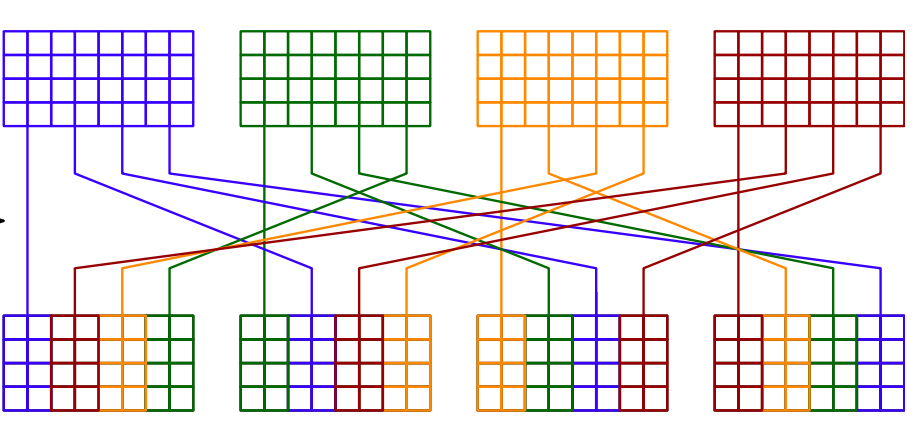
\includegraphics[width=10cm]{128.png} 
\end{center}
\begin{center}
    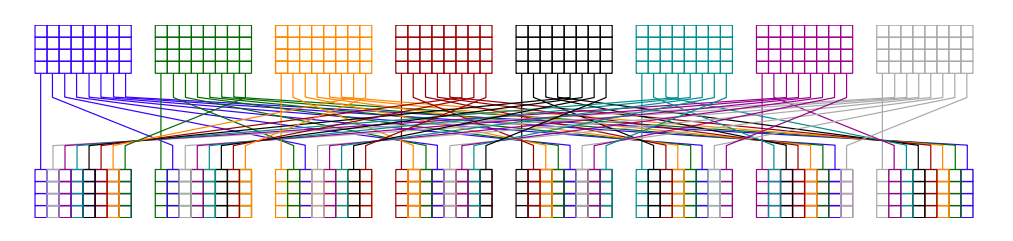
\includegraphics[scale = 0.4]{256.png} 
\end{center}

\subsection{Key and constant addition}
Up until now, we have done nothing to make the ciphertext dependent on the key. So to do this, we add the key to the state. Because we want every round to be different, we also add a round-specific constant value.\\
The Mysterion block cipher has no key schedule. In every round, the same key is added to the state.




\section{Security Analysis}
% \subsection{Attacks}
\subsection{Boomerang Attack}
This is a special type of Differential Cryptanalysis. The basic idea of this attack is to find two differentials for the two sub ciphers $C_0$ and $C_1$ obtained from cipher $C$ such that $C=C_{0} \circ C_{1}$ instead of finding one single differential for $C$. Since shorter differentials have more better probabilities, this might improve the results for the attacker.
Now to find the best differential probability of the a boomerang distinguisher, lets use 2 pre established theorems from paper $^{[9]}$ : \\ \textbf{Theorem :}  Four rounds of Mysterion-128 has at least 45 active S-boxes.  \\
\textbf{Theorem :} Four rounds of Mysterion-256 has at least 81 active S-boxes. \\
Therefore we have :  \\
For 128 bit : \\
$$\text{Pr}_{diff}(4R) \leq \text{Pr}_{diff}^{max}(Sbox)^{45} = (2^{-2})^{45} = 2^{-90} $$
$$\implies \text{Pr}_{diff}^{max}(8R) = \text{Pr}_{diff}(4R) *\text{Pr}_{diff}(4R)  = 2^{-90}*2^{-90} = 2^{-180}  
$$
the Pr obtained is way less that  brute force probability ($2^{128}$). \\
Therefore, 8 round 128 bit Mysterion is secure against Boomerang Attack.  \\ \\
Similarly, now coming to 256 bit Mysterion : \\
We use the theorem 2 above to find the max differential prob that can be obtained : 
$$\text{Pr}_{diff}^{max}(8R) = \text{Pr}_{diff}(4R) *\text{Pr}_{diff}(4R)  = 2^{-81*2}*2^{-81*2} = 2^{-324} >> 2^{-256} 
$$
the Pr obtained is way less that  brute force probability ($2^{256}$). \\
Therefore, 8 round 256 bit Mysterion is secure against Boomerang Attack.  \\ \\
Therefore Mysterion Cipher is secure against Boomerang Attack.
\subsection{Integral Attack}

Considering a collection of chosen plaintexts of m-bytes and their corresponding ciphertexts, integral attacks tries to extract information about the key by observing the sum of ciphertext values. Block ciphers based on SPNs can be tried with this attack with great efficiency. For AES, we may find integral property upto 4 rounds, and then we can mount this attack from 7-9 rounds depending on the key size. But for Mysterion after we find integral property for 4 rounds, we remain with sufficient security margin for the full cipher, since there are 12 and 16 rounds for Mysterion -128 and Mysterion-256. 
\\\\
In EUROCRYPT 2015 division property was introduced. It allows to construct more efficient integral distinguishers exploiting the limited algebraic degree of reduced ciphers. However Mysterion still has sufficient security margins for this attack also.

\subsection{Invariant subspace Attack}
\textbf{General Abstraction:} \\
Let us consider an n-bit iterative block cipher, with round function $R_k$ where,\\
$R_k$ : $\mathbb{F}_2^n$ X $\mathbb{F}_2^n$ $\rightarrow$ $\mathbb{F}_2^n$ , such that $R_k (x) = E(x + k)$ , with E as an n-bit permutation.\\
If there exists a subspace $U$ $\subseteq$ $\mathbb{F}_2^n $ and two constants $c$, $d \in \mathbb{F}_2^n$ such that $E(U + c) = U + d$, then for a round key $k = u + c + d$ with $u \in U$, the following holds:
\begin{center}
    $R_k(U + d) = E((U + d) + (u + c + d)) = E(u + c) = U + d$.
\end{center}
i.e. the round function maps the affine subspace $U + d$ onto itself. If all round
keys are in $k \in U + (c + d)$ , then this property is iterative over arbitrary number of rounds.\\

\begin{center}
    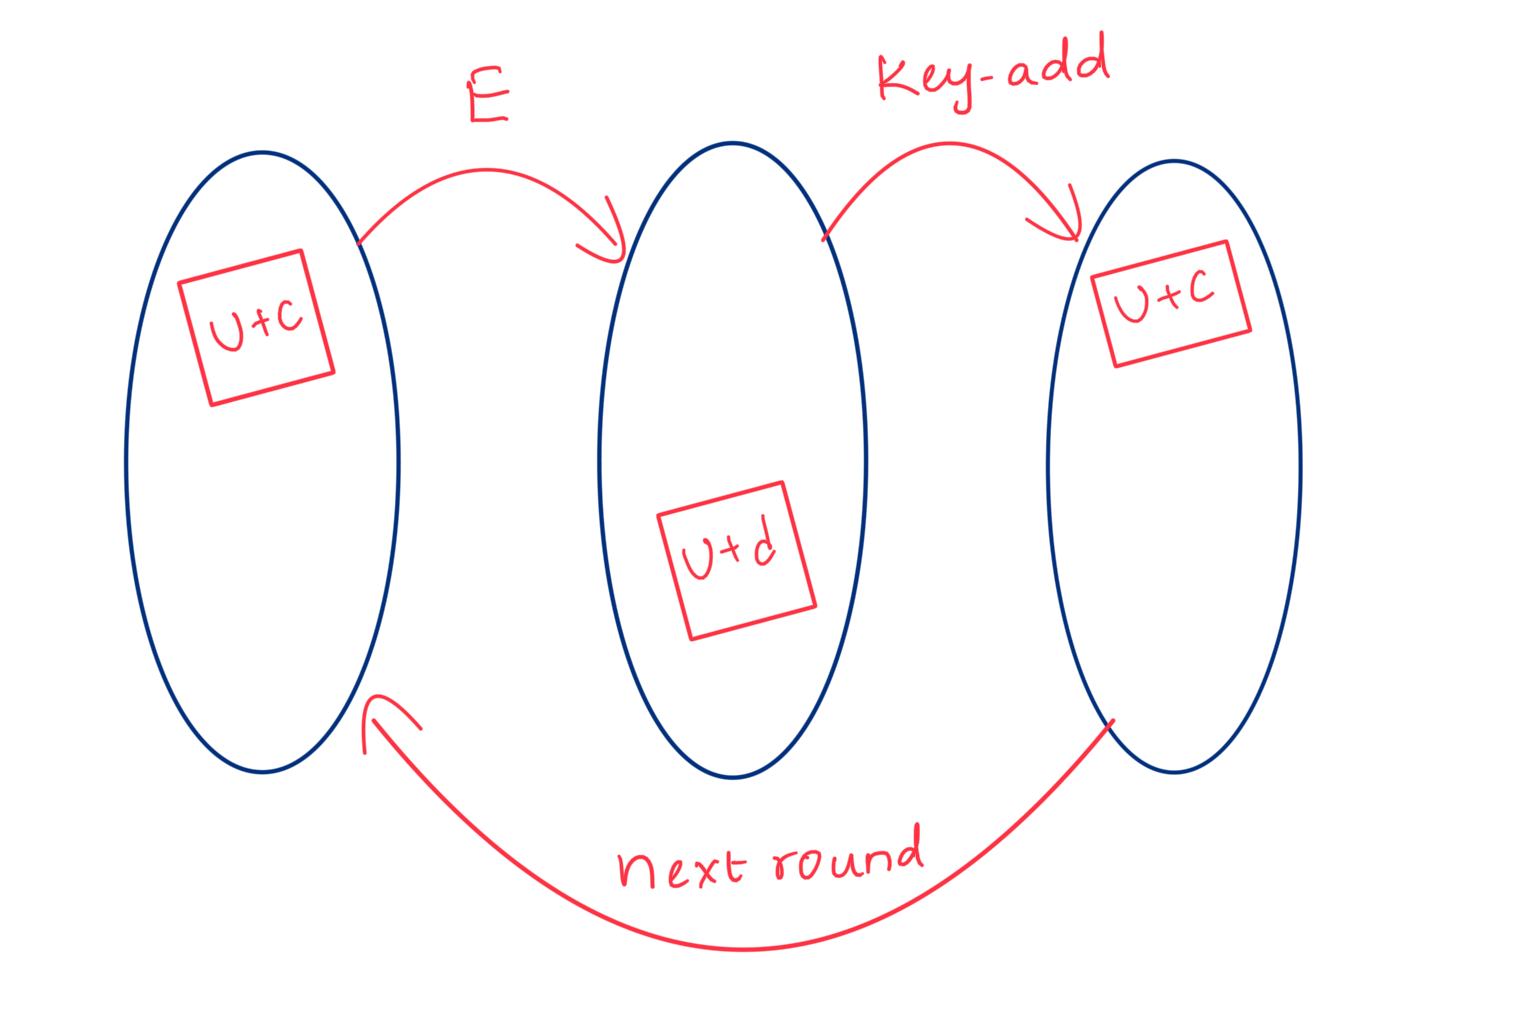
\includegraphics[width=10cm]{ISA.png}
\end{center}

LS Design models are vulnerable to this attack . This was identified by performing an exhaustive analysis on a 32 bit block.
By adding the \emph{Shift columns}  operation to LS design models (which are called as XLS models) ,this attack can no longer be done . Because, the shift columns operation prevents the propagation of subspace found for the L-box with high probability.\\ 

Hence , Mysterion being an XLS design model is resistant to invariant subspace attacks even with sparse round constants.

\section{Conclusion}
% We would however argue that the paper and the reference implementation are all a bit vague and hard to grasp. With respect to other papers, this paper could have been a lot clearer in our opinion. It almost feels like the cipher was not proposed to be actually implemented and used, as it was sometimes ambiguous and left out certain details that were crucial for implementing (like the composition of the state when applying the S-box or the definition of the round constants).
Mysterion is an example that block ciphers can be simple yet powerful and secure. XLS-design based models of ciphers have sufficient security margins for physical attacks. However grasping L-box and a few more concepts posed as a challenge to us. Implementations show that the Mysterion is very fast and is apt for lightweight uses. Although Mysterion-256 is still a bit misty to us we have been successful in implementing a working Mysterion-128 cipher. 

\section{Links}
\begin{enumerate}
    \item \href{https://github.com/Meghana-12/Mysterion}{Implementation Source Code Link}
		\item \href{https://colab.research.google.com/drive/1bmUl7wT4U13XY6n8cB2sV-f5cAsr0_vV?usp=sharing}{Google Collab Link}
		\item \href{ https://mysterion-tool.herokuapp.com/}{Online Tool Link}
		\item  \href{https://github.com/RotonEvan/mysterious-ions}{Online Tool Source code}
\end{enumerate}

%%%% 8. BILBIOGRAPHY %%%%
\bibliographystyle{alpha}
\bibliography{abbrev3,crypto,biblio}
\begin{thebibliography}{9} 
% \begin{enumerate}
  \bibitem{1}\url{https://dsprenkels.com/mysterion.html} 
   \bibitem{2} \url{https://link.springer.com/chapter/10.1007/978-3-662-46706-0_2}
   \bibitem{3}\url{https://www.researchgate.net/profile/Francois-Xavier_Standaert/publication/297725067_Improving_the_security_and_efficiency_of_block_ciphers_based_on_LS-designs/links/5c50199da6fdccd6b5d1a888/Improving-the-security-and-efficiency-of-block-ciphers-based-on-LS-designs.pdf}
   \bibitem{4} \url{https://en.wikipedia.org/wiki/Finite_field}
   \bibitem{5} \url{https://en.wikipedia.org/wiki/Companion_matrix}
   \bibitem{6}\url{https://en.wikipedia.org/wiki/MDS_matrix}
    \bibitem{7} \url{https://en.wikipedia.org/wiki/BCH_code}
    \bibitem{8} \url{https://perso.uclouvain.be/fstandae/PUBLIS/157b.pdf}
    \bibitem{9} \url{https://perso.uclouvain.be/fstandae/PUBLIS/157.pdf}
    \bibitem{10} \url{https://www.cryptolux.org/index.php/Lightweight_Block_Ciphers}
%   \end{enumerate}
\end{thebibliography}
%%%% NOTES
% - Download abbrev3.bib and crypto.bib from https://cryptobib.di.ens.fr/
% - Use bilbio.bib for additional references not in the cryptobib database.
%   If possible, take them from DBLP.

% \section{\textbf{TODO}}

% conclusion  \\

\end{document}
